\documentclass{article}
\usepackage{graphicx} % Required for inserting images
\usepackage{float} % Pour avoir des images au bon endroit du texte
\usepackage{hyperref} % pour insérer des hyper liens
\hypersetup{
    colorlinks=true,     
    urlcolor=blue,
    }
\usepackage[a4paper, margin=1in]{geometry}
\usepackage{amsmath} % pour le modulo

\title{Rapport de projet IN104 : Bobail en C}
\author{AUBRY Julie, BORDEAU Pierre}
\date{Mai 2024}

\begin{document}

\maketitle

Les instructions pour exécuter le code sont disponibles sur \href{https://github.com/pierrebrd/IN104_Projet/tree/main}{Github}, dans le Readme.

\section{Présentation du projet}

\subsection{Le jeu de bobail}

Le bobail est un jeu de plateau d'origine africaine. Sur un plateau de 5x5, chaque joueur possède 5 pions, au début de la partie tous dans une colonne extrémale. Un pion particulier, le bobail, est placé au centre du plateau.


Les joueurs peuvent gagner en ramenant le bobail dans la colonne où étaient leurs pions au début de la partie. Lorsque le bobail est encerclé et ne peut plus bouger, il y a également victoire. Le joueur responsable de l'encerclement est vainqueur.


A chaque tour, le joueur déplace d'abord le bobail puis un de ses pions. Au premier tour, on ne déplace pas le bobail.
Le bobail peut se déplacer d'une case selon l'une des huit directions cardinales : nord, nord-est, est, sud-est, sud, sud-ouest, ouest, nord-ouest.
Les autres pions se déplacent en ligne droite selon chacune des huit directions, jusqu'à rencontrer un obstacle (autre pion ou bord du plateau).

\subsection{Les exigences du projet}

Ce projet consiste à implémenter en C le jeu de bobail avec une interface en ligne de commande. Il est d'abord demandé de permettre à deux joueurs de jouer, puis d'implémenter une intelligence artificielle.



\section{Jeu en 1 v 1}

\subsection{Choix concernant la grille de jeu}

Nous avons choisi que, à tout moment, l'état du jeu sera contenu dans une structure que nous avons appelé {\tt struct jeu\_t} qui contient la grille et la liste des abscisses et des ordonnées de tous les pions.


Nous avons choisi de représenter la grille de jeu comme une matrice 5x5, implémentée avec un {\tt int** grille}
Cela permet de modéliser facilement quelle case est occupée par quoi, en représentant par :
\\- 0 : case vide
\\- 1 : case occupée par un pion du joueur 1
\\- 2 : case occupée par un pion du joueur 2
\\- 3 : case occupée par le bobail


Convention de l'indexation de la grille :
lignes i croissant de haut en bas
colonnes j croissant de gauche à droite


Les listes {\tt int* x\_pions} et {\tt int* y\_pions} enregistrent les positions des pions : les 5 premiers éléments sont les pions du joueur 1, les 5 suivants ceux du joueur 2, et le onzième élément correspond au bobail.


L'avantage de cette double représentation de l'état du jeu est qu'on profite à la fois de la simplicité de la manipulation de la grille pour les déplacements, et de la liste des positions des pions, ce qui évite de rechercher les pions dans la grille quand on en a besoin (pour l'IA notamment).
\\
\\
Nous avons du représenter la grille de jeu dans le terminal, d'une manière compréhensible par deux joueurs qui s'affrontent, et visuellement agréable. A ces fins, on utilise des caractères Unicode pour faire la grille  \href{https://en.wikipedia.org/wiki/List_of_Unicode_characters}{(catégorie "Box Drawing")}.
Pour afficher les pions, on utilise des cercles dont on change la couleur.

\begin{figure}[H]
    \centering
    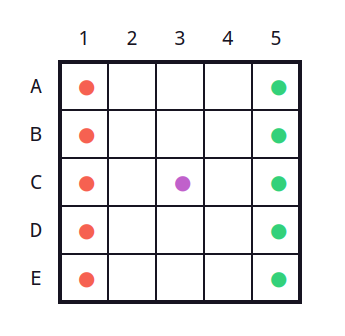
\includegraphics[width=0.5\linewidth]{grille.png}
    \caption{Exemple de l'affichage}
    \label{fig:1}
\end{figure}

\subsection{Choix concernant le déplacement}

Pour connaître le coup que le joueur souhaite effectuer, on lui demande d'entrer la position initiale et la position finale en "format bataille navale". Premièrement, cela nous a semblé plus intuitif que les directions cardinales, et cela a facilité l'implémentation du déplacement.
\\ \\On obtient l'input en ligne de commande avec {\tt scanf()}. Nous avons choisi d'accepter uniquement les réponses du type "LettreChiffre" avec Lettre qui vaut A B C D ou E et chiffre qui vaut 1 2 3 4 ou 5. Si l'input n'est pas de ce format, on redemande à l'utilisateur une nouvelle réponse. Il a été envisagé de prendre en compte les réponses non-valides mais compréhensibles telles que "c5 ou "C 5", mais les difficultés techniques n'en valaient pas la peine.
\\ \\ Concernant le déplacement en lui même, il s'effectue en ligne droite horizontalement, verticalement ou diagonalement, d'une case pour le bobail et jusqu'à rencontrer un obstacle pour les autres pions. Grâce à la méthode choisie pour l'input utilisateur, on sait que le déplacement ne "sort" jamais de la grille. Cependant, on a dû s'assurer que le déplacement suit bien une des directions autorisées.
\\ Une fois la direction de déplacement obtenue, on bouge le pion une case à la fois en s'assurant que la case suivante n'est ni occupée, ni le bord du plateau. Au total, on a relevé six types de déplacements invalides possibles :
\\1) le bobail bouge au 1er tour, ou reste immobile à un coup qui n'est pas le 1er
\\2) il n'y a pas de déplacement de pion (initial = final)
\\3) la direction n'est pas une diagonale, une verticale ou une horizontale
\\4) une case est déja occupée sur le chemin
\\5) le bobail est déplacé de plus de 1 case
\\6) on n'est pas allé au bout du déplacement du pion (ie jusqu'à rencontrer un obstacle)
\\\\Nous avons créé une fonction {\tt int legit(jeu\_t *jeu, int ia, int ja, int ib, int jb, int type\_pion)} qui renvoie 0 si le  coup est valide, et un nombre entre 1 et 6 sinon (suivant la raison de l'invalidité). Par ailleurs, lors de l'implémentation d'IA, nous avons associé à chaque coup possible un entier entre 0 et 359 qui sera explicité dans le paragraphe suivant. Nous avons eu besoin de savoir si un coup était valide avec en entrée l'indice du coup, et pour cela nous avons créé {\tt int legit\_direction(jeu\_t *jeu, int indice\_coup, int joueur, int tour)}
\\ \\Grâce à l'implémentation matricielle de {\tt int** jeu->grille}, il est aisé de déplacer un pion :  il suffit de remplir sa case initiale par 0, et sa case finale par la valeur du pion. Plus tard dans le projet, on a ajouté les listes {\tt int* x\_pions} et {\tt int* y\_pions} dans lesquelles on doit également prendre en compte le déplacement.


\subsection{Condition de victoire}

Nous avons créé la fonction {\tt int victoire(jeu\_t *jeu, int joueur)} qui donne le vainqueur dans l'état actuel du jeu, où le joueur s'apprête à jouer : 1 si joueur 1 a gagné, 2 si joueur 2 a gagné, 0 si personne n'a gagné.
\\ Grâce à l'implémentation matricielle, il est facile de vérifier si le bobail est dans la première colonne (victoire du joueur 1) ou dans le dernière colonne (victoire du joueur 2).
\\ Pour savoir si le bobail est bloqué, on veut savoir s'il pourrait effectuer un déplacement vers une de ses huit cases voisines. Au lieu de vérifier cela manuellement, nous réemployons la fonction {\tt legit}. Si les huit voisins sont occupés, alors le bobail est bloqué et le joueur qui vient de jouer a gagné.

\begin{figure}[H]
    \centering
    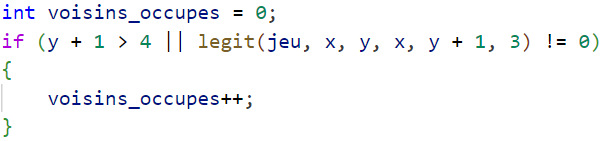
\includegraphics[width=0.5\linewidth]{victoire.png}
    \caption{Voyons si le bobail peut aller dans la case au sud}
    \label{fig:1.2}
\end{figure}

\subsection{Partie entre deux joueurs humains}

La fonction {\tt jeu1v1()} permet à deux joueurs de jouer l'un contre l'autre. Nous avons soigné l'aspect visuel en affichant les règles, et en utilisant la fonction {\tt sleep()} pour afficher le texte au fur et à mesure. Pour cette raison, le programme ne peut fonctionner que sous Linux avec {\tt \#include <unistd.h>}.


\section{Première intelligence artificielle : coups aléatoires}

Pour utiliser des algorithmes d'intelligence artificielle, il a d'abord fallu implémenter des fonctions permettant de jouer des coups de manière aléatoire.
Il faut pour cela définir la manière de représenter un "coup" que peut joueur un joueur à son tour.

Nous avons choisi de représenter les coups possibles d'un joueur comme des entiers de 0 à 359. Chaque entier correspond à un unique coup possible.
\\- le bobail peut se déplacer dans 8 directions, où ne pas bouger (c'est le cas au premier tour), ce qui fait 9 possibilités. on repère donc la direction du bobail par un entier de 0 à 8.
\\- Le joueur doit déplacer un de ses 5 pions. On les indices de 0 à 4 pour le joueur 1 et de 5 à 9 pour le joueur 2.
\\- Le pion choisi peut se déplacer dans 8 directions, indicées de 0 à 7.


Ainsi, on obtient l'entier correspondant à un coup :
% $$coup = direction\_bobail * (5*8) + numero\_pion * 8 direction\_pion$$
% Je trouvais ta formule bizarre
$$coup = direction\_bobail * 40 + (numero\_pion\mod 5) * 8 + direction\_pion$$

\begin{figure}[H]
    \centering
    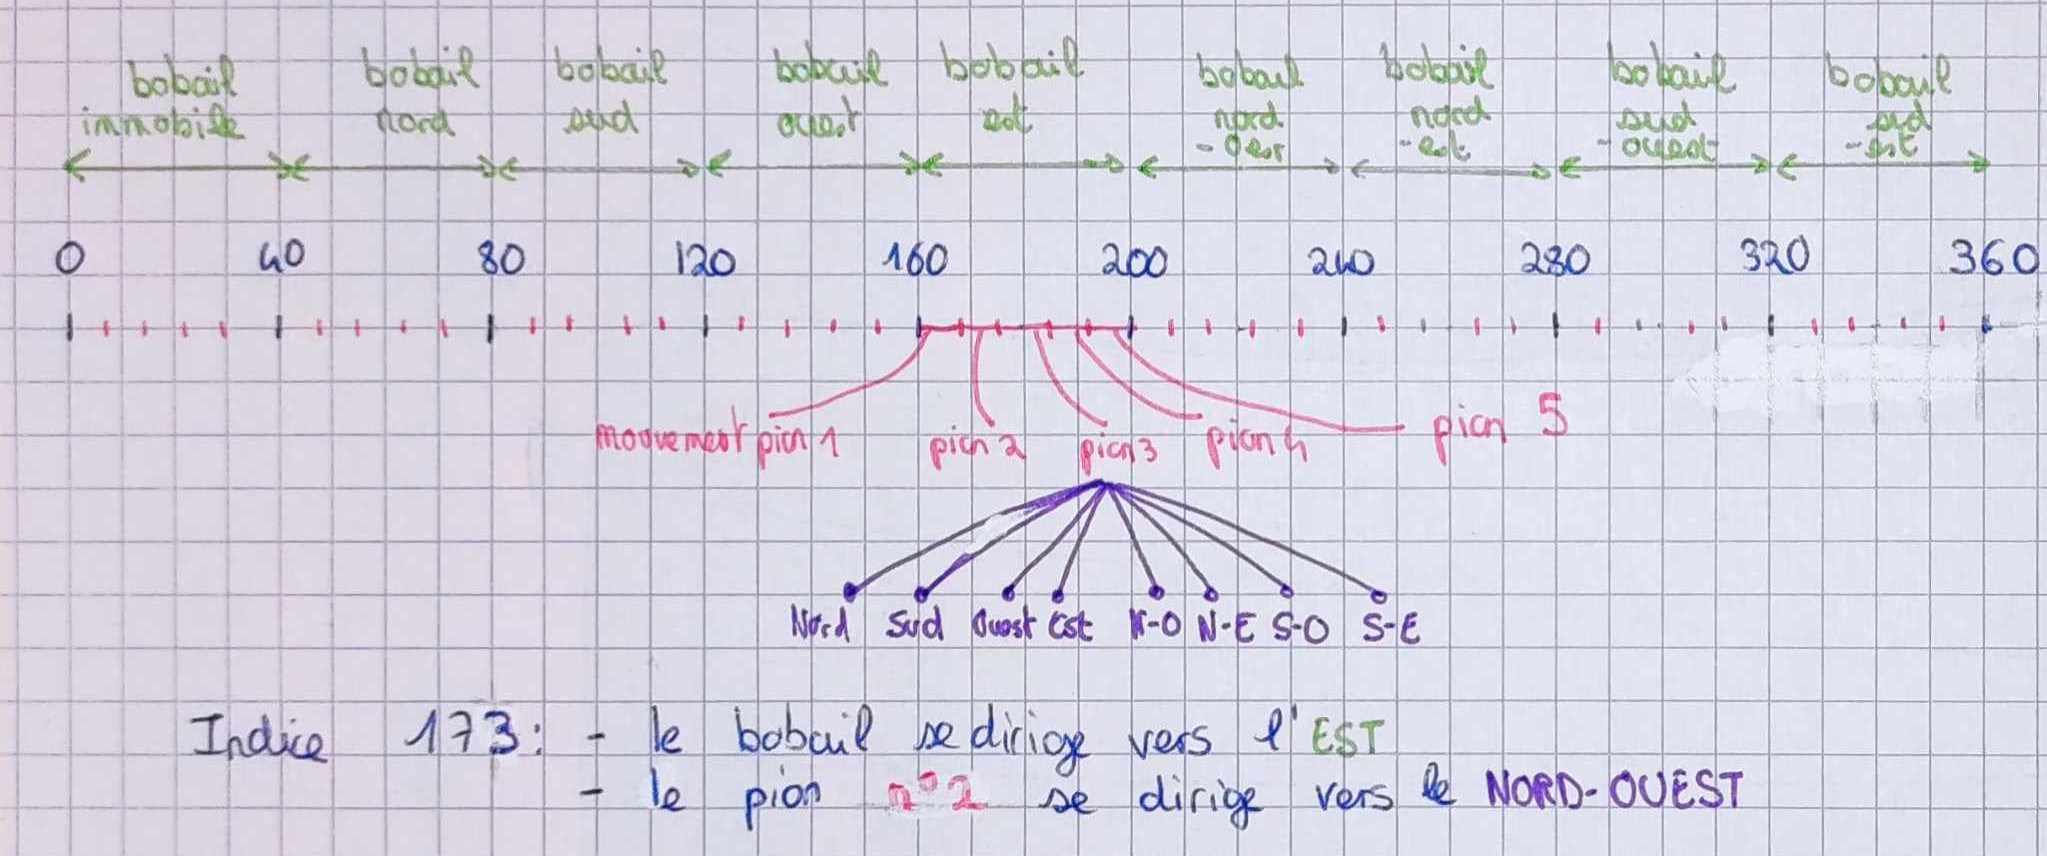
\includegraphics[width=1\linewidth]{explication_indice_coup.jpeg}
    \caption{Explication de l'indice du coup}
    \label{fig:1.5}
\end{figure}

Ensuite, on peut analyser si des coup peuvent être joués avec la fonction {\tt legit\_direction(jeu\_t *jeu, int indice\_coup, int joueur, int tour)}, les jouer avec {\tt jouer\_coup(jeu\_t *jeu, int joueur, int indice\_coup)}, et générer un coup aléatoire avec  {\tt coup\_hasard(jeu\_t *jeu, int joueur, int tour)}
\\Nous avons donc pu créer les fonctions  {\tt jeu1vIA\_aleatoire()} et {\tt jeuIAvIA\_aleatoire()}
qui permettent de joueur contre un ordinateur qui joue aléatoirement, et de regarder deux ordinateurs jouer aléatoirement l'un contre l'autre.



\section{Implémentation de l'algorithme MCTS}

Maintenant que l'on peut jouer des coups de manière aléatoire, nous implémentons un algorithme d'intelligence artificielle pour que l'ordinateur choisisse un coup à son avantage. Le problème est qu'à chaque tour, il y a énormément de possibilités de coup possibles (environ 150). Il est donc compliqué d'explorer l'entièreté de l'arbre des possibles à partir d'un certain état de jeu.

Nous avons choisi d'implémenter un algorithme inspiré de celui de Monte Carlo Tree Search (MCTS). Quand l'IA doit choisir un coup, elle explore tous les coups possibles plusieurs milliers de fois : elle joue le coup, puis elle simule la partie aléatoirement jusqu'à le fin. Si elle gagne, elle incrémente un compteur de succès. Finalement, elle choisit le jeu qui, au bout de plusieurs milliers de parties aléatoires, est le plus avantageux.

Cet algorithme, implémenté dans {\tt MCTS(jeu\_t *jeu, int joueur, int tour, int nbr\_simulations)} est déjà assez efficace, un joueur humain peut facilement perdre face à l'IA.

Cependant, comme l'algorithme simule des parties aléatoires après son coup, il ne voit pas forcément si un coup, d'apparence avantageux quand l'adversaire joue aléatoirement, permet en fait à l'adversaire de jouer un coup malin que le mènera à la victoire. Ainsi, l'IA fait des coups qui lui paraissent avantageux mais qui la mènent en fait à une défaite rapide.

Nous avons donc pu créer les fonctions  {\tt jeu1vIA()} et {\tt jeuIAvIA()}
qui permettent de joueur contre une IA utilisant MCTS, et de regarder deux IA jouer l'une contre l'autre.

\begin{figure}[H]
    \centering
    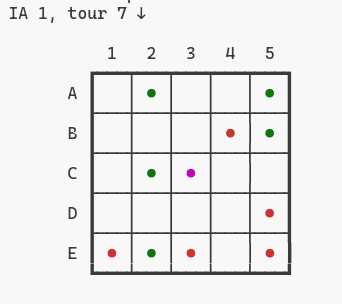
\includegraphics[width=0.3\linewidth]{ia v1 -2.png}
    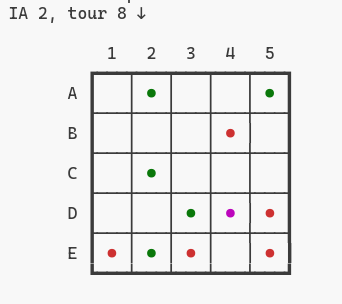
\includegraphics[width=0.3\linewidth]{ia v1 -1.png}
    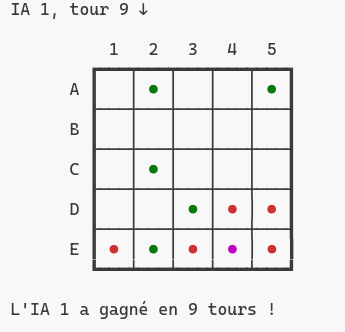
\includegraphics[width=0.3\linewidth]{ia v1.png}
    \caption{L'IA 2 pense jouer un coup avantageux, mais permet en fait à l'IA 1 de gagner instantanément}
    \label{fig:2}
\end{figure}




\section{Tentative d'amélioration de MCTS}

Nous avons ensuite voulu améliorer MCTS en utilisant la récursivité : Admettons que ce soit à J1 de jouer. Il va choisir le meilleur de ses coups, non pas en simulant des parties aléatoires après son coup, mais en considérant que l'adversaire choisit son meilleur coup grâce à MCTS, puis en terminant la partie de manière aléatoire. On a ainsi un algorithme {\tt MCTS\_improved(jeu\_t *jeu, int joueur, int tour, int nb\_explorations)}, qui a une récursivité d'ordre 1.

L'algorithme est ainsi plus intelligent car il fait attention à ne pas jouer un coup qui mènerait directement son adversaire à la victoire.

Nous avons donc pu créer les fonctions  {\tt jeu1vIA\_improved()} et {\tt jeuIAvIA\_improved()}
qui permettent de joueur contre une IA utilisant MCTS amélioré, et de regarder deux IA jouer l'une contre l'autre.

\section{Comparaison des algorithmes}

Pour évaluer si l'algorithme récursif d'ordre 1 plus intelligent que l'algorithme initial, nous avons fait jouer les deux IA l'une contre l'autre en simulant 2400 parties : 1200 parties où l'IA améliorée joue en premier, et 1200 où elle joue en deuxième.

\begin{table} [H]
    \centering
    \begin{tabular}{|c|c|c|c|}
        \hline
                                        & IA améliorée  & IA classique & Total de parties \\ \hline
        L'IA améliorée joue en premier  & 1033 (86,1\%) & 136 (11,3\%) & 1200             \\ \hline
        L'IA améliorée joue en deuxième & 811 (67,6\%)  & 308 (23,7\%) & 1200             \\ \hline
        Total                           & 1844 (76,8\%) & 444 (18,5\%) & 2400             \\
        \hline
    \end{tabular}
    \caption{Nombre de victoires en fonction de l'IA utilisée}
    \label{tab:1}
\end{table}

On observe ainsi que l'IA améliorée est plus performante que L'IA classique, en particulier quand elle joue en premier. Nous nous sommes donc demandés si il était plus avantageux de joueur en premier.

Nous avons alors simulé 1200 parties dans lesquelles les deux IA utilisent l'algorithme amélioré, pour savoir si celle qui joue en premier est avantagée.

\begin{table} [H]
    \centering
    \begin{tabular}{|c|c|c|c|}
        \hline
        IA 1         & IA 2         & Matchs nuls  & Total de parties \\ \hline
        340 (28,3\%) & 293 (24,4\%) & 567 (47,3\%) & 1200             \\
        \hline
    \end{tabular}
    \caption{Nombre de victoires en fonction de qui joue en premier}
    \label{tab:2}
\end{table}

L'IA qui joue en premier semble gagner plus souvent, mais généralement la partie finit en match nul (on l'arrête au bout de 100 tours car la situation n'évolue plus). Les deux IA évitent de jouer des coups dangereux et ainsi la partie stagne, souvent dans une configuration comme celle-ci :

\begin{figure}[H]
    \centering
    \includegraphics[width=0.3\linewidth]{bloqué.png}
    \caption{Situation classique de jeu qui stagne}
    \label{fig:3}
\end{figure}


%% Annexe ?

\section{Organisation du travail}

Nous avons travaillé en utilisant Github. Afin de ne pas avoir de problèmes de merge, nous travaillons chacun sur des fichiers différents et faisons des commits réguliers. Ainsi le code est décomposé en de très nombreux fichiers

Nous nous répartissions au fur et à mesure le travail, et avons utilisé Notion pour organiser l'avancée du projet.

\begin{figure}[H]
    \centering
    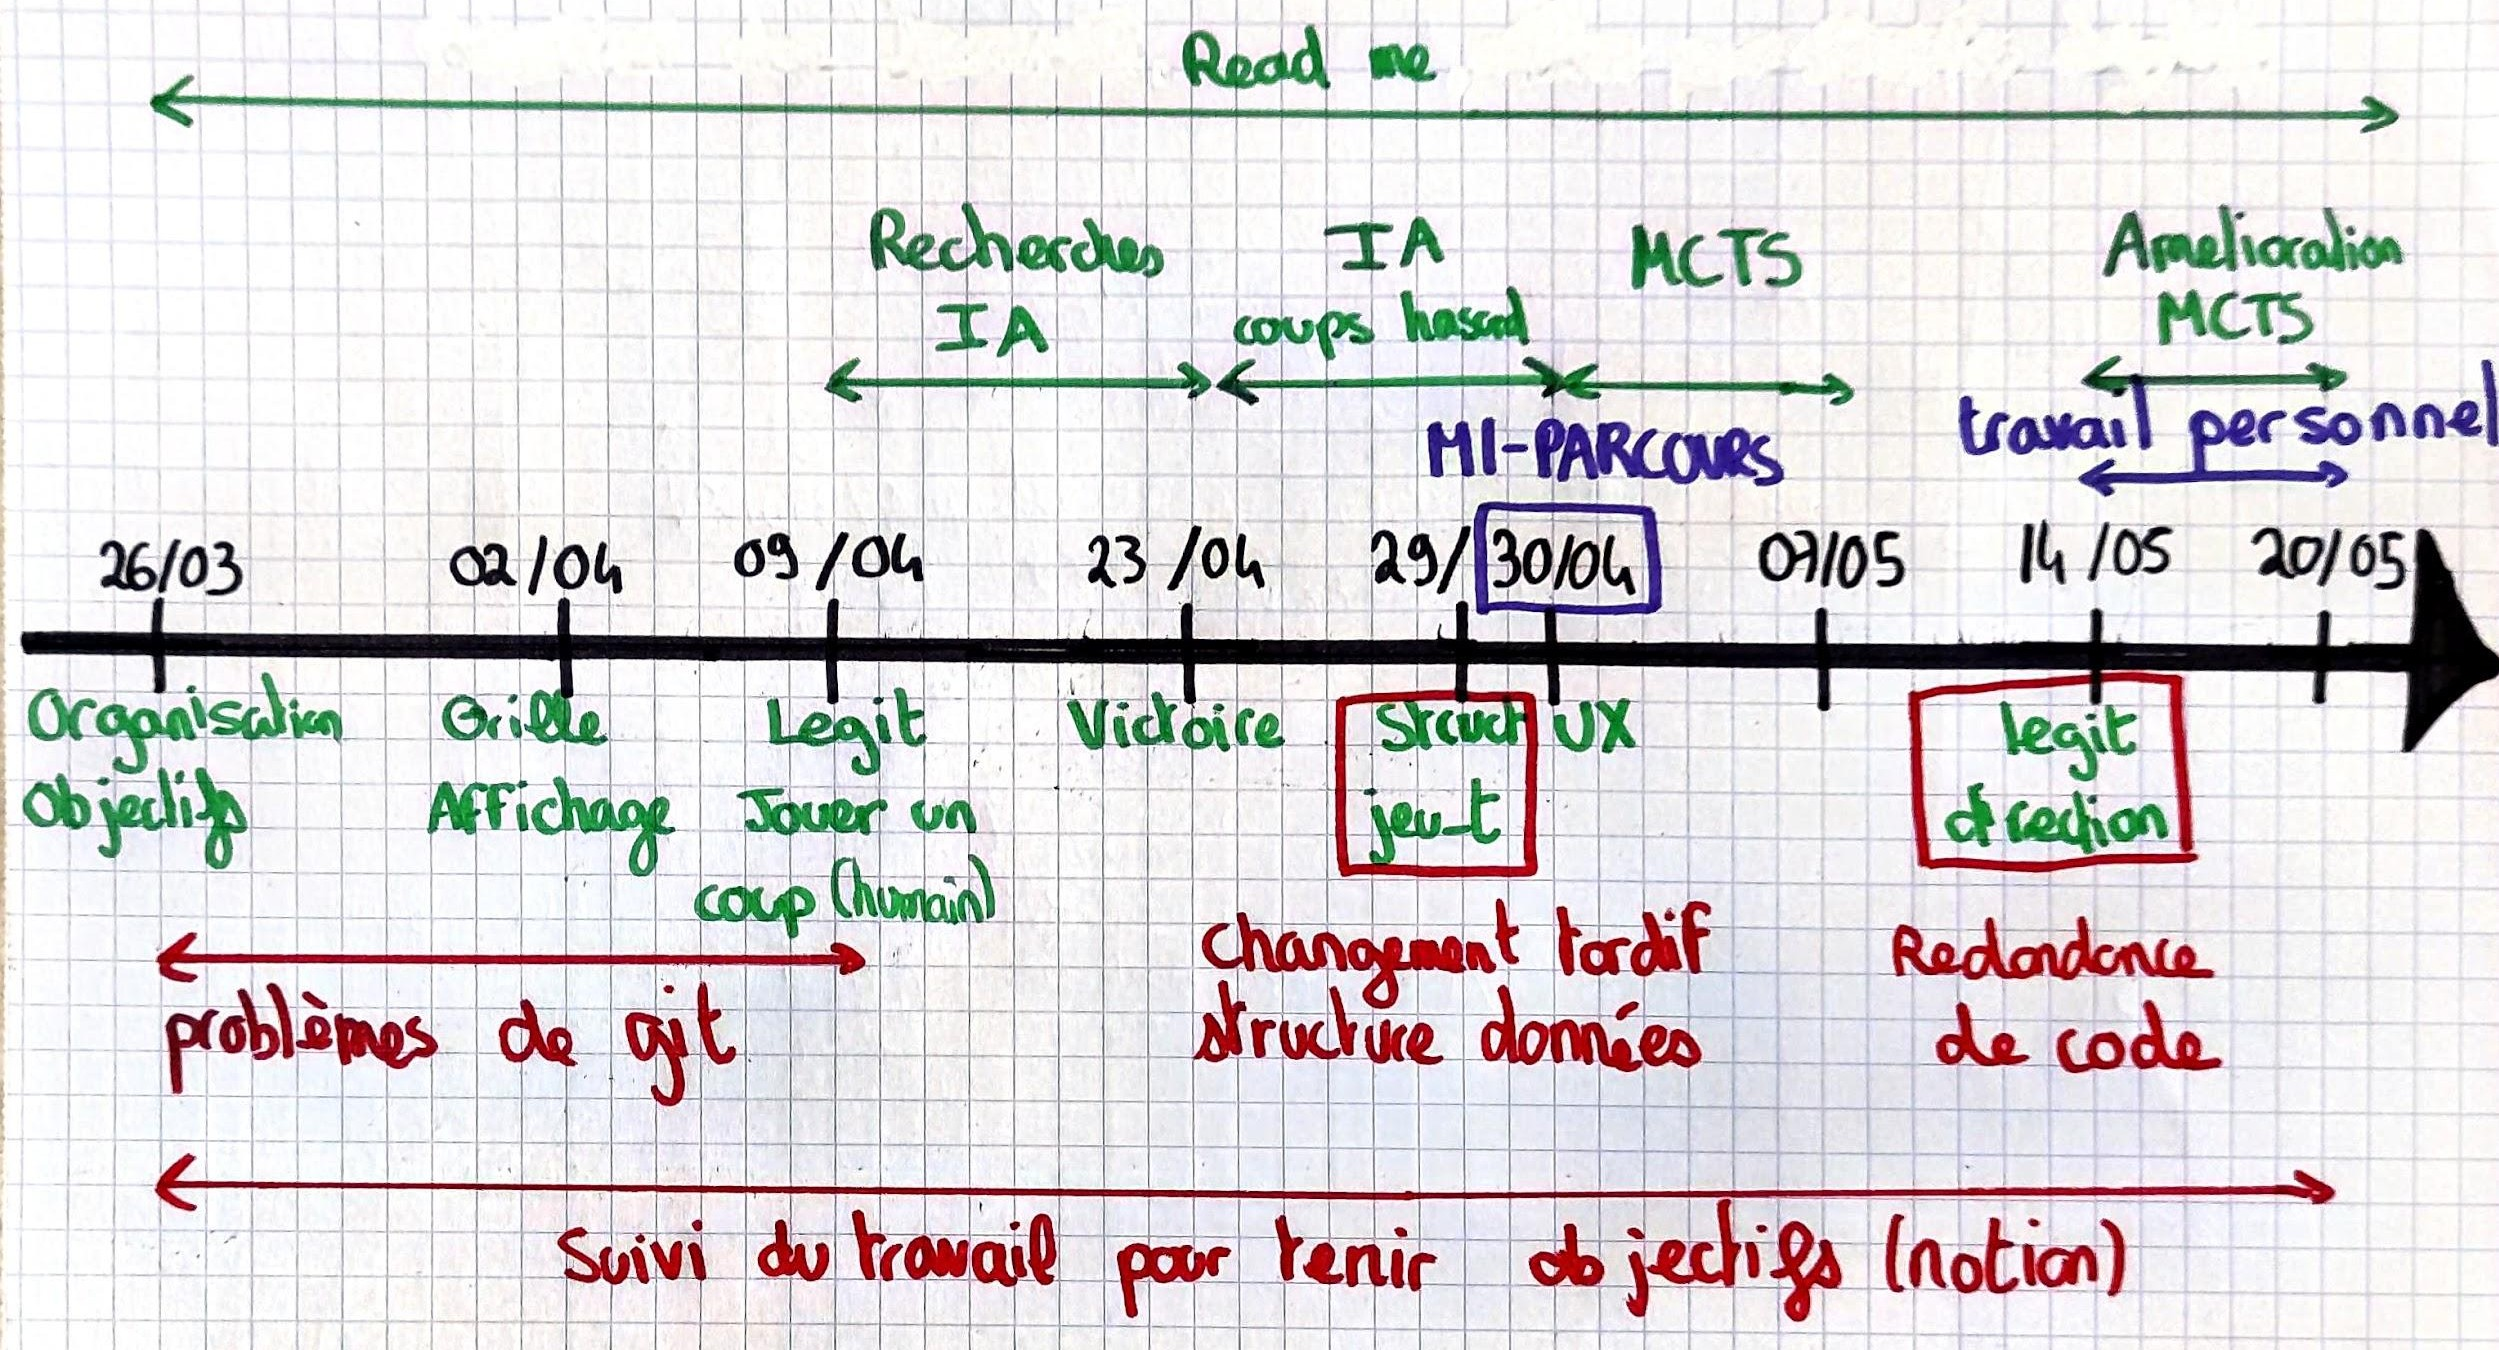
\includegraphics[width=0.7\linewidth]{timeline.jpg}
    \caption{Timeline du projet}
    \label{fig:3}
\end{figure}


Nous avons rencontré plusieurs difficulté durant le projet. D'abord, il a fallu comprendre le fonctionnement de git, nous avions au début beaucoup de "merge conflicts". Nous avons donc séparé notre code en de nombreux fichiers et utilisé une branche temporaire, IA, pour coder les algorithmes liés à l'IA.

Au début du projet, l'état du jeu était seulement représenté par {\tt int** grille}, mais quand nous avons réfléchi aux algorithmes d'intelligence artificielle, nous nous sommes rendu compte que ce n'était pas une bonne idée de rechercher à chaque fois la position du bobail et des pions dans la grille, nous avons donc plutôt opté pour une structure {\tt struct jeu\_t}. En plus de {\tt int** grille}, il contient les listes {\tt x\_pions} et {\tt y\_pions}. Elles stockent respectivement les abscisses et les ordonnées des pions, indicés de 0 à 4 pour le joueur 1, 5 à 9 pour le joueur 2, et indice 10 pour le bobail.

Nous avons aussi rencontré un problème avec lors de la génération de coups aléatoires : parfois, la partie se bloquait et un joueur ne pouvait bouger aucun pion, et le programme tournait alors à l'infini. Nous avons donc ajouté un compteur d'itérations : quand le programme ne trouve pas de coups possibles après, il met fin à la partie sans qu'il n'y ait de gagnant (Figure 4).

Enfin nous avons du résoudre de nombreux bugs au fur et à mesure de l'avancée du projet. Pour les détecter, nous utilisions essentiellement des {\tt printf} pour afficher les différentes variables, et {\tt afficher(jeu\_t *jeu);} pour afficher la grille.

\begin{figure}[H]
    \centering
    \includegraphics[width=0.3\linewidth]{problème.png}
    \caption{Jeu bloqué : le joueur vert ne peut déplacer aucun de ses pions.}
    \label{fig:4}
\end{figure}






\section{Architecture des fichiers}

Une documentation précise des différentes fonction est accessible dans les fichiers .h du code source. Voici une description des différents fichiers et de leur utilité :

\begin{itemize}
    \item {\tt affichage.c/h } contient les fonctions permettant d'afficher dans le terminal la grille représentant l'état du jeu (Pierre).
    \item {\tt deplacement.c/h } contient les fonctions demandant à un joueur de choisir un coup en donnant les coordonnées des anciennes et nouvelles positions et en vérifiant que l'entrée est correct (Julie) et les fonctions permettant de changer l'état du jeu à partir des données d'un coup (Pierre).
    \item {\tt hasard.c/h} contient la fonction permettant de générer un coup aléatoire (Pierre).
    \item {\tt IA.c/h} contient la fonction permettant d'explorer une branche aléatoirement jusqu'à la fin de la partie ainsi que l'algorithme MCTS classique (Pierre), et l'algorithme MCTS récursif (Julie).
    \item {\tt initialisation.c/h} contient les fonctions permettant d'initialiser le {\tt struct jeu\_t} en début de partie, de le détruire, ou de copier le contenu d'un jeu dans un autre (Julie). Le fichier .h contient aussi la définition de {\tt struct jeu\_t} et de {\tt enum direction\_t}.
    \item {\tt jeu1v1.c/h}, {\tt jeu1vIA.c/h} et {\tt jeuIAvIA.c/h} contiennent les fonctions permettant de jouer à deux joueurs, contre un IA ou de regarder deux IA s'affronter (Pierre).
    \item {\tt legit.c/h} contient les fonctions permettant de savoir si un coup est légal à partir des nouvelles et anciennes positions des pions (Pierre) ou de l'indice entier représentant un coup (Julie).
    \item {\tt UX.c/h} permet d'afficher les règles, ce qui est utilisé dans {\tt main.c} (Julie)
    \item {\tt victoire.c/h} contient la fonction permettant de déterminer si la partie est terminée et renvoie le gagnant le cas échéant. (Julie)

    \item {\tt main.c} permet de lancer le jeu et de demander à l'utilisateur le mode de jeu qui lui convient. (Pierre)
    \item {\tt test\_comparaisonIA.c} contient le programme utilisée pour comparer les deux types d'intelligence artificielle. (Pierre)
    \item {\tt test\_jouerenpremier.c} contient le programme comparant la proportion de victoire entre l'IA qui joue en premier et celle qui joue en deuxième. (Pierre)
    \item Les autres fichiers tests étaient utiles pour tester les fonctions au fur et à mesure de l'avancée du projet.
\end{itemize}







\end{document}
